%%%%%%%%%%%%%%%%%%%%%%%%%%%%%%%%%%%%%%%%%
% Programming/Coding Assignment
% LaTeX Template
%
% This template has been downloaded from:
% http://www.latextemplates.com
%
% Original author:
% Ted Pavlic (http://www.tedpavlic.com)
%
% Note:
% The \lipsum[#] commands throughout this template generate dummy text
% to fill the template out. These commands should all be removed when 
% writing assignment content.
%
% This template uses a Perl script as an example snippet of code, most other
% languages are also usable. Configure them in the "CODE INCLUSION 
% CONFIGURATION" section.
%
%%%%%%%%%%%%%%%%%%%%%%%%%%%%%%%%%%%%%%%%%

%----------------------------------------------------------------------------------------
%	PACKAGES AND OTHER DOCUMENT CONFIGURATIONS
%----------------------------------------------------------------------------------------

\documentclass{article}
\usepackage{amsmath}
\usepackage{fancyhdr} % Required for custom headers
\usepackage{lastpage} % Required to determine the last page for the footer
\usepackage{extramarks} % Required for headers and footers
\usepackage[usenames,dvipsnames]{color} % Required for custom colors
\usepackage{graphicx} % Required to insert images
\usepackage{subcaption}
\usepackage{listings} % Required for insertion of code
\usepackage{courier} % Required for the courier font
\usepackage{lipsum} % Used for inserting dummy 'Lorem ipsum' text into the template

% % % % % % % % %
\usepackage{listings}
\usepackage{color}

\definecolor{dkgreen}{rgb}{0,0.6,0}
\definecolor{gray}{rgb}{0.5,0.5,0.5}
\definecolor{mauve}{rgb}{0.58,0,0.82}

\lstset{frame=tb,
  language=Python,
  aboveskip=3mm,
  belowskip=3mm,
  showstringspaces=false,
  columns=flexible,
  basicstyle={\small\ttfamily},
  numbers=none,
  numberstyle=\tiny\color{gray},
  keywordstyle=\color{blue},
  commentstyle=\color{dkgreen},
  stringstyle=\color{mauve},
  breaklines=true,
  breakatwhitespace=true,
  tabsize=3
}
% % % % % % % % %
% Margins
\topmargin=-0.45in
\evensidemargin=0in
\oddsidemargin=0in
\textwidth=6.5in
\textheight=9.0in
\headsep=0.25in

\linespread{1.1} % Line spacing

% Set up the header and footer
\pagestyle{fancy}
\lhead{\hmwkAuthorName} % Top left header
\chead{\hmwkClass\ (\hmwkClassTime): \hmwkTitle} % Top center head
\rhead{\firstxmark} % Top right header
\lfoot{\lastxmark} % Bottom left footer
\cfoot{} % Bottom center footer
\rfoot{Page\ \thepage\ of\ \protect\pageref{LastPage}} % Bottom right footer
\renewcommand\headrulewidth{0.4pt} % Size of the header rule
\renewcommand\footrulewidth{0.4pt} % Size of the footer rule

\setlength\parindent{0pt} % Removes all indentation from paragraphs

%----------------------------------------------------------------------------------------
%	CODE INCLUSION CONFIGURATION
%----------------------------------------------------------------------------------------

\definecolor{MyDarkGreen}{rgb}{0.0,0.4,0.0} % This is the color used for comments
\lstloadlanguages{Perl} % Load Perl syntax for listings, for a list of other languages supported see: ftp://ftp.tex.ac.uk/tex-archive/macros/latex/contrib/listings/listings.pdf
\lstset{language=Perl, % Use Perl in this example
        frame=single, % Single frame around code
        basicstyle=\small\ttfamily, % Use small true type font
        keywordstyle=[1]\color{Blue}\bf, % Perl functions bold and blue
        keywordstyle=[2]\color{Purple}, % Perl function arguments purple
        keywordstyle=[3]\color{Blue}\underbar, % Custom functions underlined and blue
        identifierstyle=, % Nothing special about identifiers                                         
        commentstyle=\usefont{T1}{pcr}{m}{sl}\color{MyDarkGreen}\small, % Comments small dark green courier font
        stringstyle=\color{Purple}, % Strings are purple
        showstringspaces=false, % Don't put marks in string spaces
        tabsize=5, % 5 spaces per tab
        %
        % Put standard Perl functions not included in the default language here
        morekeywords={rand},
        %
        % Put Perl function parameters here
        morekeywords=[2]{on, off, interp},
        %
        % Put user defined functions here
        morekeywords=[3]{test},
       	%
        morecomment=[l][\color{Blue}]{...}, % Line continuation (...) like blue comment
        numbers=left, % Line numbers on left
        firstnumber=1, % Line numbers start with line 1
        numberstyle=\tiny\color{Blue}, % Line numbers are blue and small
        stepnumber=5 % Line numbers go in steps of 5
}

% Creates a new command to include a perl script, the first parameter is the filename of the script (without .pl), the second parameter is the caption
\newcommand{\perlscript}[2]{
\begin{itemize}
\item[]\lstinputlisting[caption=#2,label=#1]{#1.pl}
\end{itemize}
}

%----------------------------------------------------------------------------------------
%	DOCUMENT STRUCTURE COMMANDS
%	Skip this unless you know what you're doing
%----------------------------------------------------------------------------------------

% Header and footer for when a page split occurs within a problem environment
\newcommand{\enterProblemHeader}[1]{
\nobreak\extramarks{#1}{#1 continued on next page\ldots}\nobreak
\nobreak\extramarks{#1 (continued)}{#1 continued on next page\ldots}\nobreak
}

% Header and footer for when a page split occurs between problem environments
\newcommand{\exitProblemHeader}[1]{
\nobreak\extramarks{#1 (continued)}{#1 continued on next page\ldots}\nobreak
\nobreak\extramarks{#1}{}\nobreak
}

\setcounter{secnumdepth}{0} % Removes default section numbers
\newcounter{homeworkProblemCounter} % Creates a counter to keep track of the number of problems

\newcommand{\homeworkProblemName}{}
\newenvironment{homeworkProblem}[1][Part \arabic{homeworkProblemCounter}]{ % Makes a new environment called homeworkProblem which takes 1 argument (custom name) but the default is "Problem #"
\stepcounter{homeworkProblemCounter} % Increase counter for number of problems
\renewcommand{\homeworkProblemName}{#1} % Assign \homeworkProblemName the name of the problem
\section{\homeworkProblemName} % Make a section in the document with the custom problem count
\enterProblemHeader{\homeworkProblemName} % Header and footer within the environment
}{
\exitProblemHeader{\homeworkProblemName} % Header and footer after the environment
}

\newcommand{\problemAnswer}[1]{ % Defines the problem answer command with the content as the only argument
\noindent\framebox[\columnwidth][c]{\begin{minipage}{0.98\columnwidth}#1\end{minipage}} % Makes the box around the problem answer and puts the content inside
}

\newcommand{\homeworkSectionName}{}
\newenvironment{homeworkSection}[1]{ % New environment for sections within homework problems, takes 1 argument - the name of the section
\renewcommand{\homeworkSectionName}{#1} % Assign \homeworkSectionName to the name of the section from the environment argument
\subsection{\homeworkSectionName} % Make a subsection with the custom name of the subsection
\enterProblemHeader{\homeworkProblemName\ [\homeworkSectionName]} % Header and footer within the environment
}{
\enterProblemHeader{\homeworkProblemName} % Header and footer after the environment
}

%----------------------------------------------------------------------------------------
%	NAME AND CLASS SECTION
%----------------------------------------------------------------------------------------

\newcommand{\hmwkTitle}{Project 4} % Assignment title
\newcommand{\hmwkDueDate}{Triangulation Matting} % Due date
\newcommand{\hmwkClass}{CSC320} % Course/class
\newcommand{\hmwkClassTime}{L0101} % Class/lecture time
\newcommand{\hmwkAuthorName}{Ramaneek Gill and Ryan D'Souza} % Your name

%----------------------------------------------------------------------------------------
%	TITLE PAGE
%----------------------------------------------------------------------------------------

\title{
\vspace{2in}
\textmd{\textbf{\hmwkClass:\ \hmwkTitle}}\\
\normalsize\vspace{0.1in}\small{\hmwkDueDate}\\
\vspace{0.1in}
\vspace{3in}
}

\author{\textbf{\hmwkAuthorName}}
%\date{} % Insert date here if you want it to appear below your name

%----------------------------------------------------------------------------------------

\begin{document}

\maketitle
\clearpage




%----------------------------------------------------------------------------------------
%	PART 1
%----------------------------------------------------------------------------------------

\begin{homeworkProblem}

\noindent
$$ 
C = 
	\begin{bmatrix}
	       C_1\\
	       C_2
	\end{bmatrix}
, \hspace{10mm} B = 
	\begin{bmatrix}
		       B_1\\
		       B_2
	\end{bmatrix} \\
$$
\\
$$C = F + (1-\alpha)B$$
$$C = F + B - B\alpha$$
$$C - B = F - B\alpha$$ 
$$\Rightarrow$$

$$
\left(\begin{matrix}
1 & 	0 & 	0 & -B^{r}_1 \\
0 & 	1 & 	0 & -B^{g}_1 \\
0 & 	0 & 	1 & -B^{b}_1 \\
1 & 	0 & 	0 & -B^{r}_2 \\
0 & 	1 & 	0 & -B^{g}_2 \\
0 & 	0 & 	1 & -B^{b}_2 \\
\end{matrix} \right) 
\left(\begin{matrix}
F_r \\
F_g \\
F_b \\
\alpha
\end{matrix}\right) = 
\left(
\begin{matrix}
  C^{r}_1  -B^{r}_1 \\
  C^{g}_1 -B^{g}_1 \\
  C^{b}_1 -B^{b}_1 \\
  C^{r}_2 -B^{r}_2 \\
  C^{g}_2-B^{g}_2 \\
  C^{b}_2-B^{b}_2 \\
\end{matrix}
\right).
$$



\end{homeworkProblem}

%----------------------------------------------------------------------------------------
%	PART 2
%----------------------------------------------------------------------------------------
\begin{homeworkProblem}

\noindent

The input images were 4 input images. 2 were composite images of a flower with a white background and other one with a black background. The two different background images (white and black) were also given. These 4 input images were used with another image (a window background) to produce a new composite image a flower as the foreground with triangulation matting.\\

\begin{figure}[h!]
        \centering
        \begin{subfigure}[b]{0.3\textwidth}
                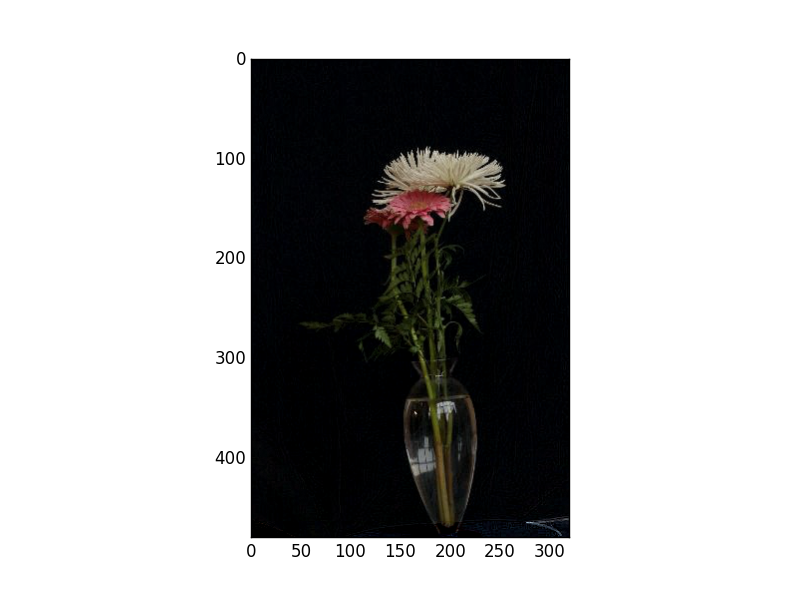
\includegraphics[width=\textwidth]{flower-foreground.png}
                \caption{The foreground computed from using two composite images with the same foreground but different backgrounds}
                \label{fig:1a}
        \end{subfigure}%
        ~
        \begin{subfigure}[b]{0.3\textwidth}
                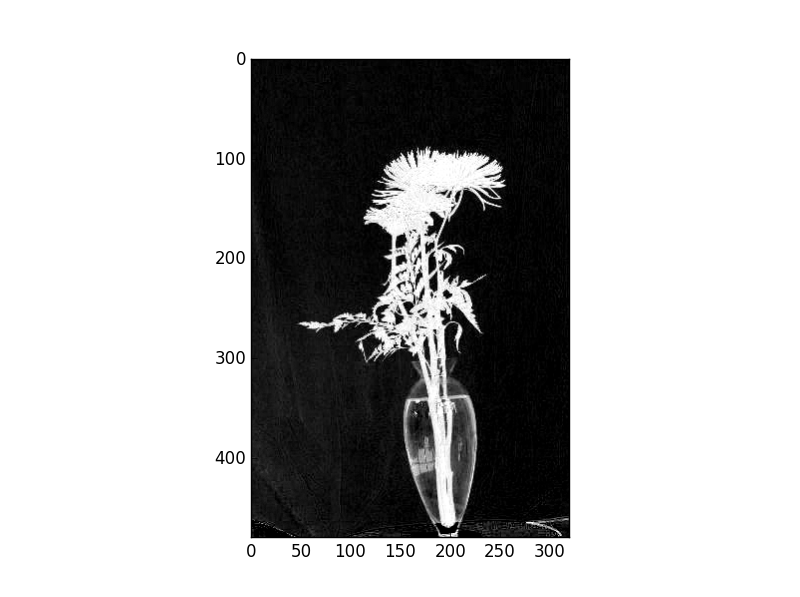
\includegraphics[width=\textwidth]{foreground-alpha-channel.png}
                \caption{The alpha channel computed}
                \label{fig:1b}
        \end{subfigure}
        ~
        \begin{subfigure}[b]{0.3\textwidth}
                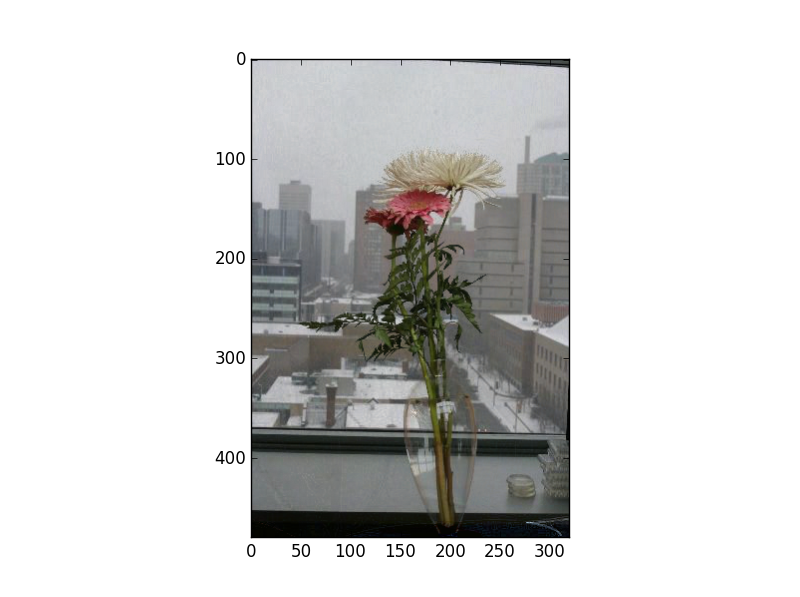
\includegraphics[width=\textwidth]{window-and-flower.png}
                \caption{The custom composite image with the same foreground but new background}
                \label{fig:1c}
        \end{subfigure}
        \caption{Images computed through the triangulation matting algorithm}\label{fig:dataset}
\end{figure}
\end{homeworkProblem}
\clearpage
%----------------------------------------------------------------------------------------
%	PART 3
%----------------------------------------------------------------------------------------
\begin{homeworkProblem}

\noindent
There is no way I can produce an image where the foreground is the exact same with two different backgrounds since I don't have a tripod, my only camera is the one included in my phone so the results will be very shaky. Below are my 5 input images and the results of the triangulation matting.\\

I got these images by doing the following:\\
1. Take a picture of a background.\\
2. Move foreground object in front of background (the mug in the figures below) and take a picture.\\
3. Change background, leave mug in same exact place and take a picture.\\
4. Remove foreground and take a picture.\\
5. Try to do all of these steps while balancing the camera (android phone) on a stable surface and try to move its angle of view as little as possible.\\
\\
The fifth step (the lack of a tripod) was the reason the output from the triangulation matting algorithm was horrible. The input image backgrounds were not as similar we want them to be since the camera can view a very different image (because of projection) when comparing the data pixel-wise. From an object recognition standpoint the input images are perfect.

\begin{figure}[h!]
        \centering
        \begin{subfigure}[b]{0.49\textwidth}
                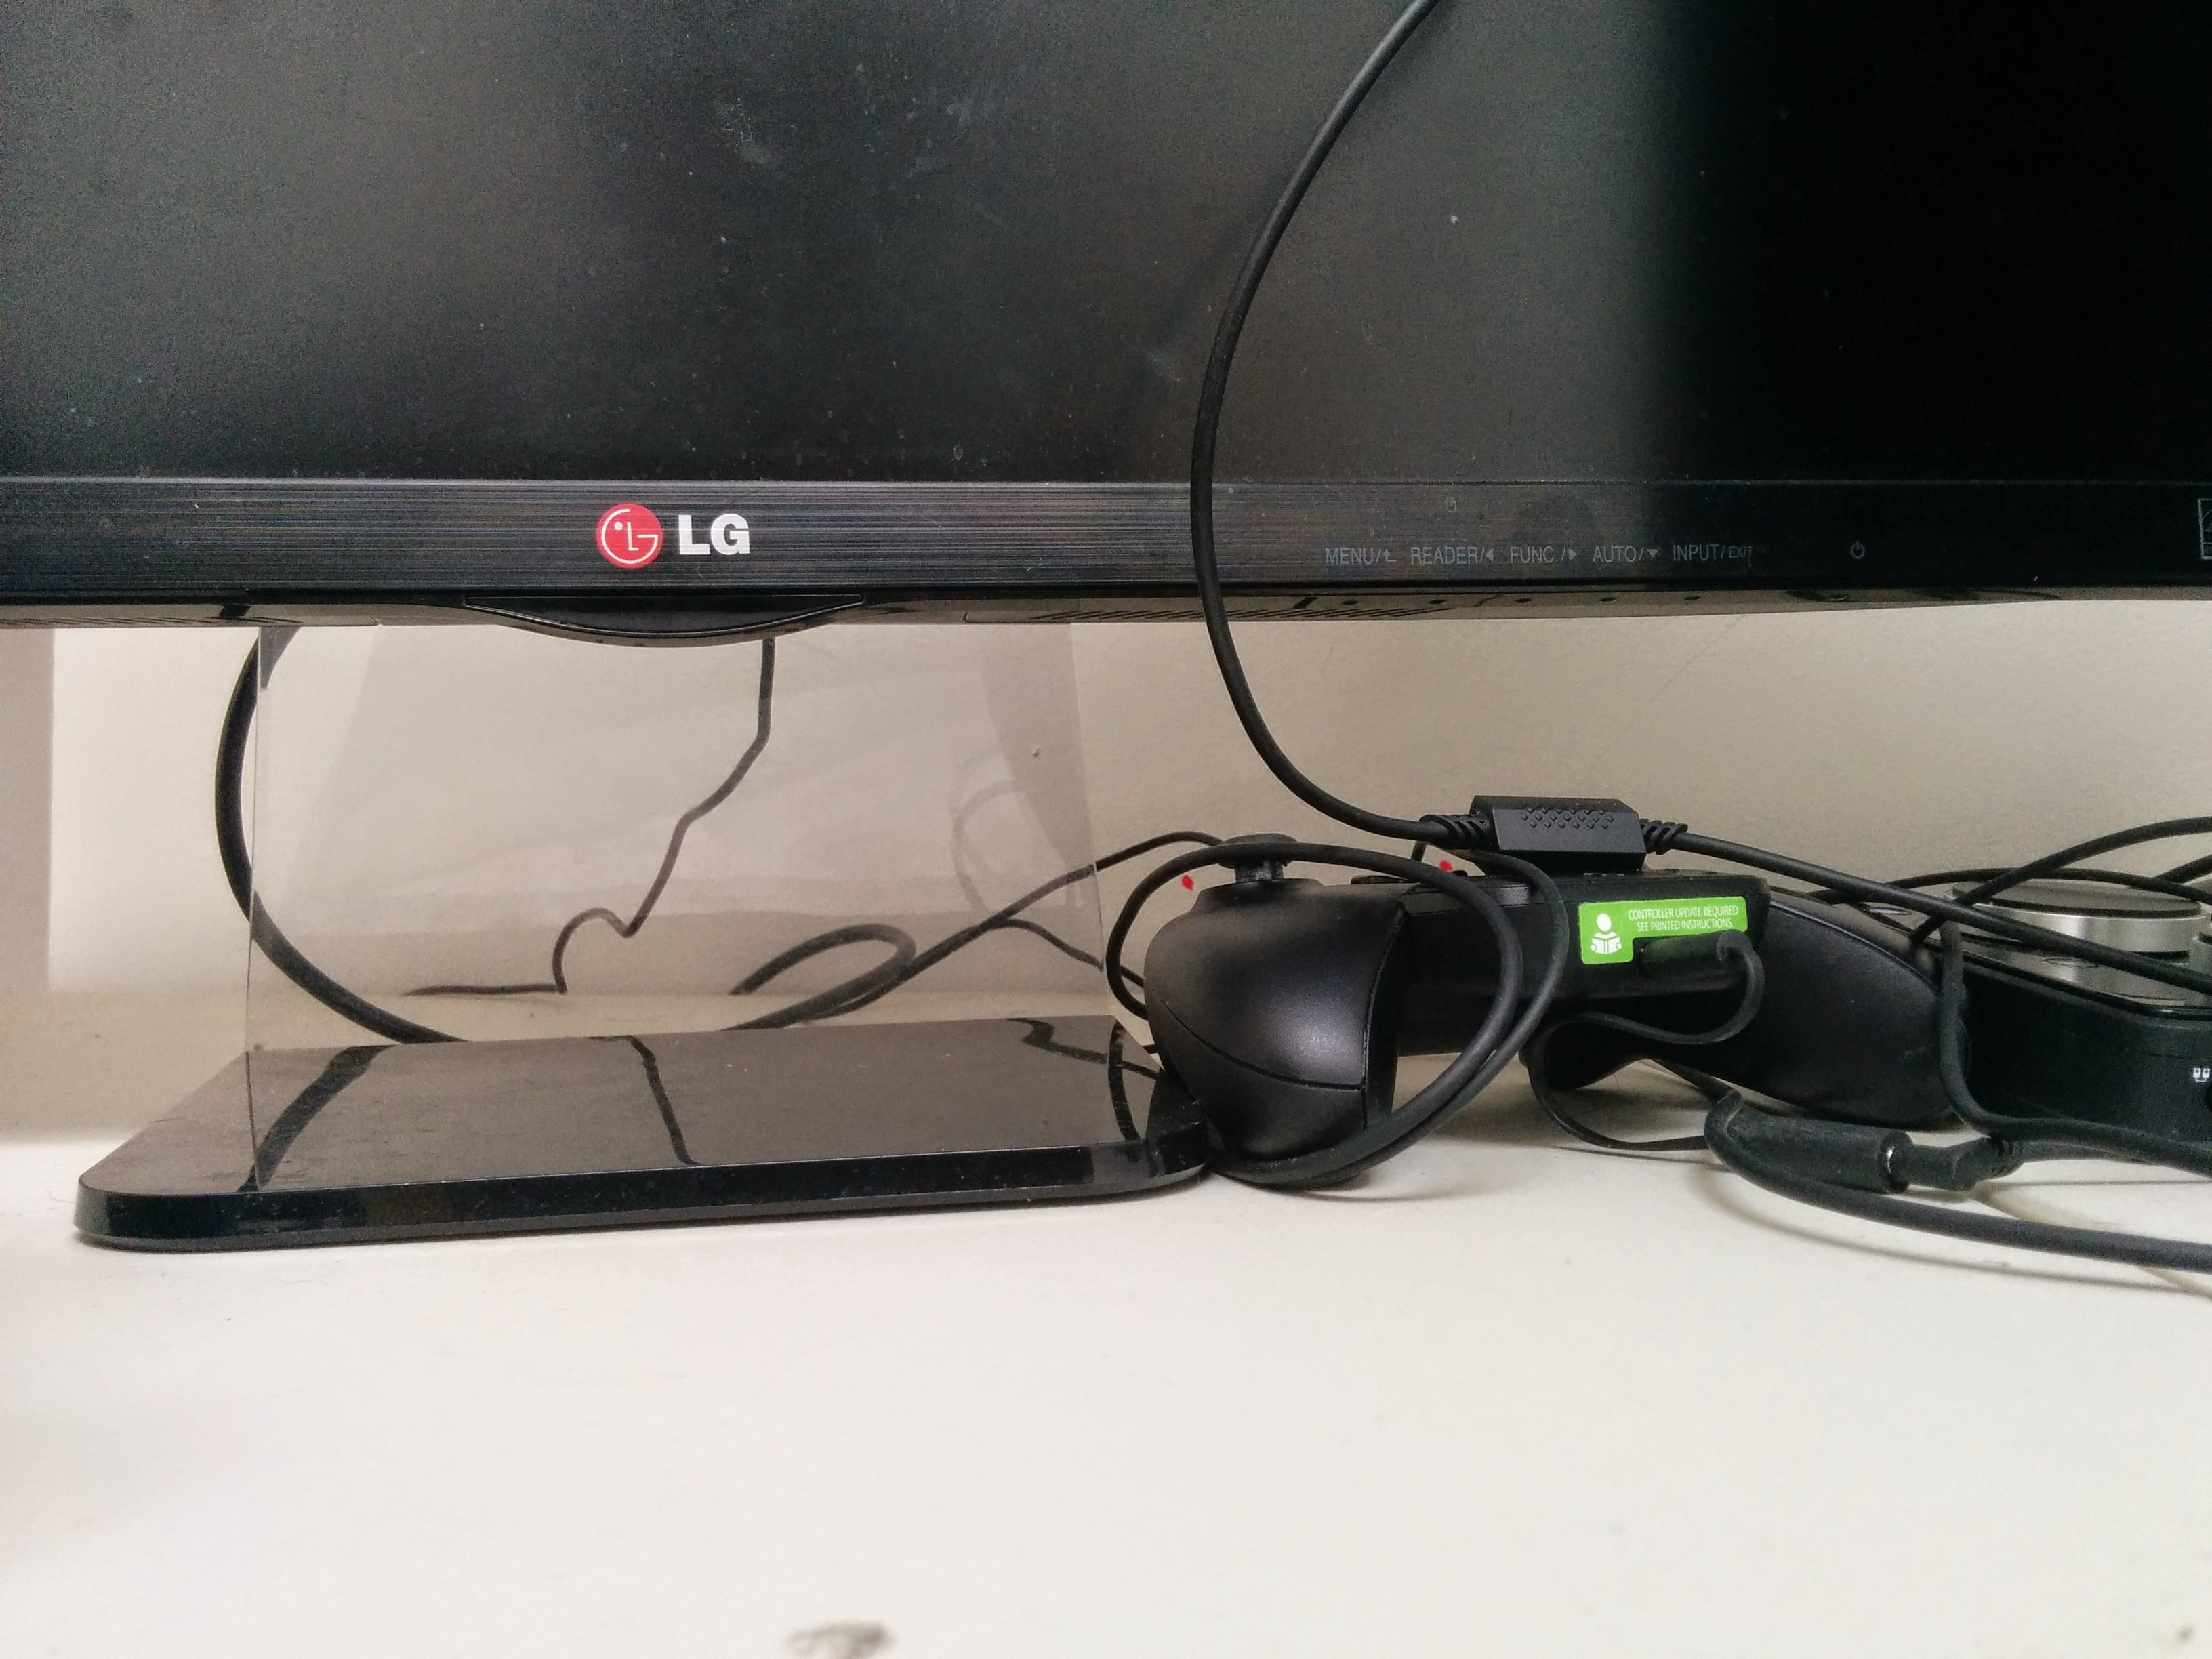
\includegraphics[width=\textwidth]{my-images/b1.jpg}
                \caption{Background 1}
                \label{fig:1a}
        \end{subfigure}%
        ~
        \begin{subfigure}[b]{0.49\textwidth}
                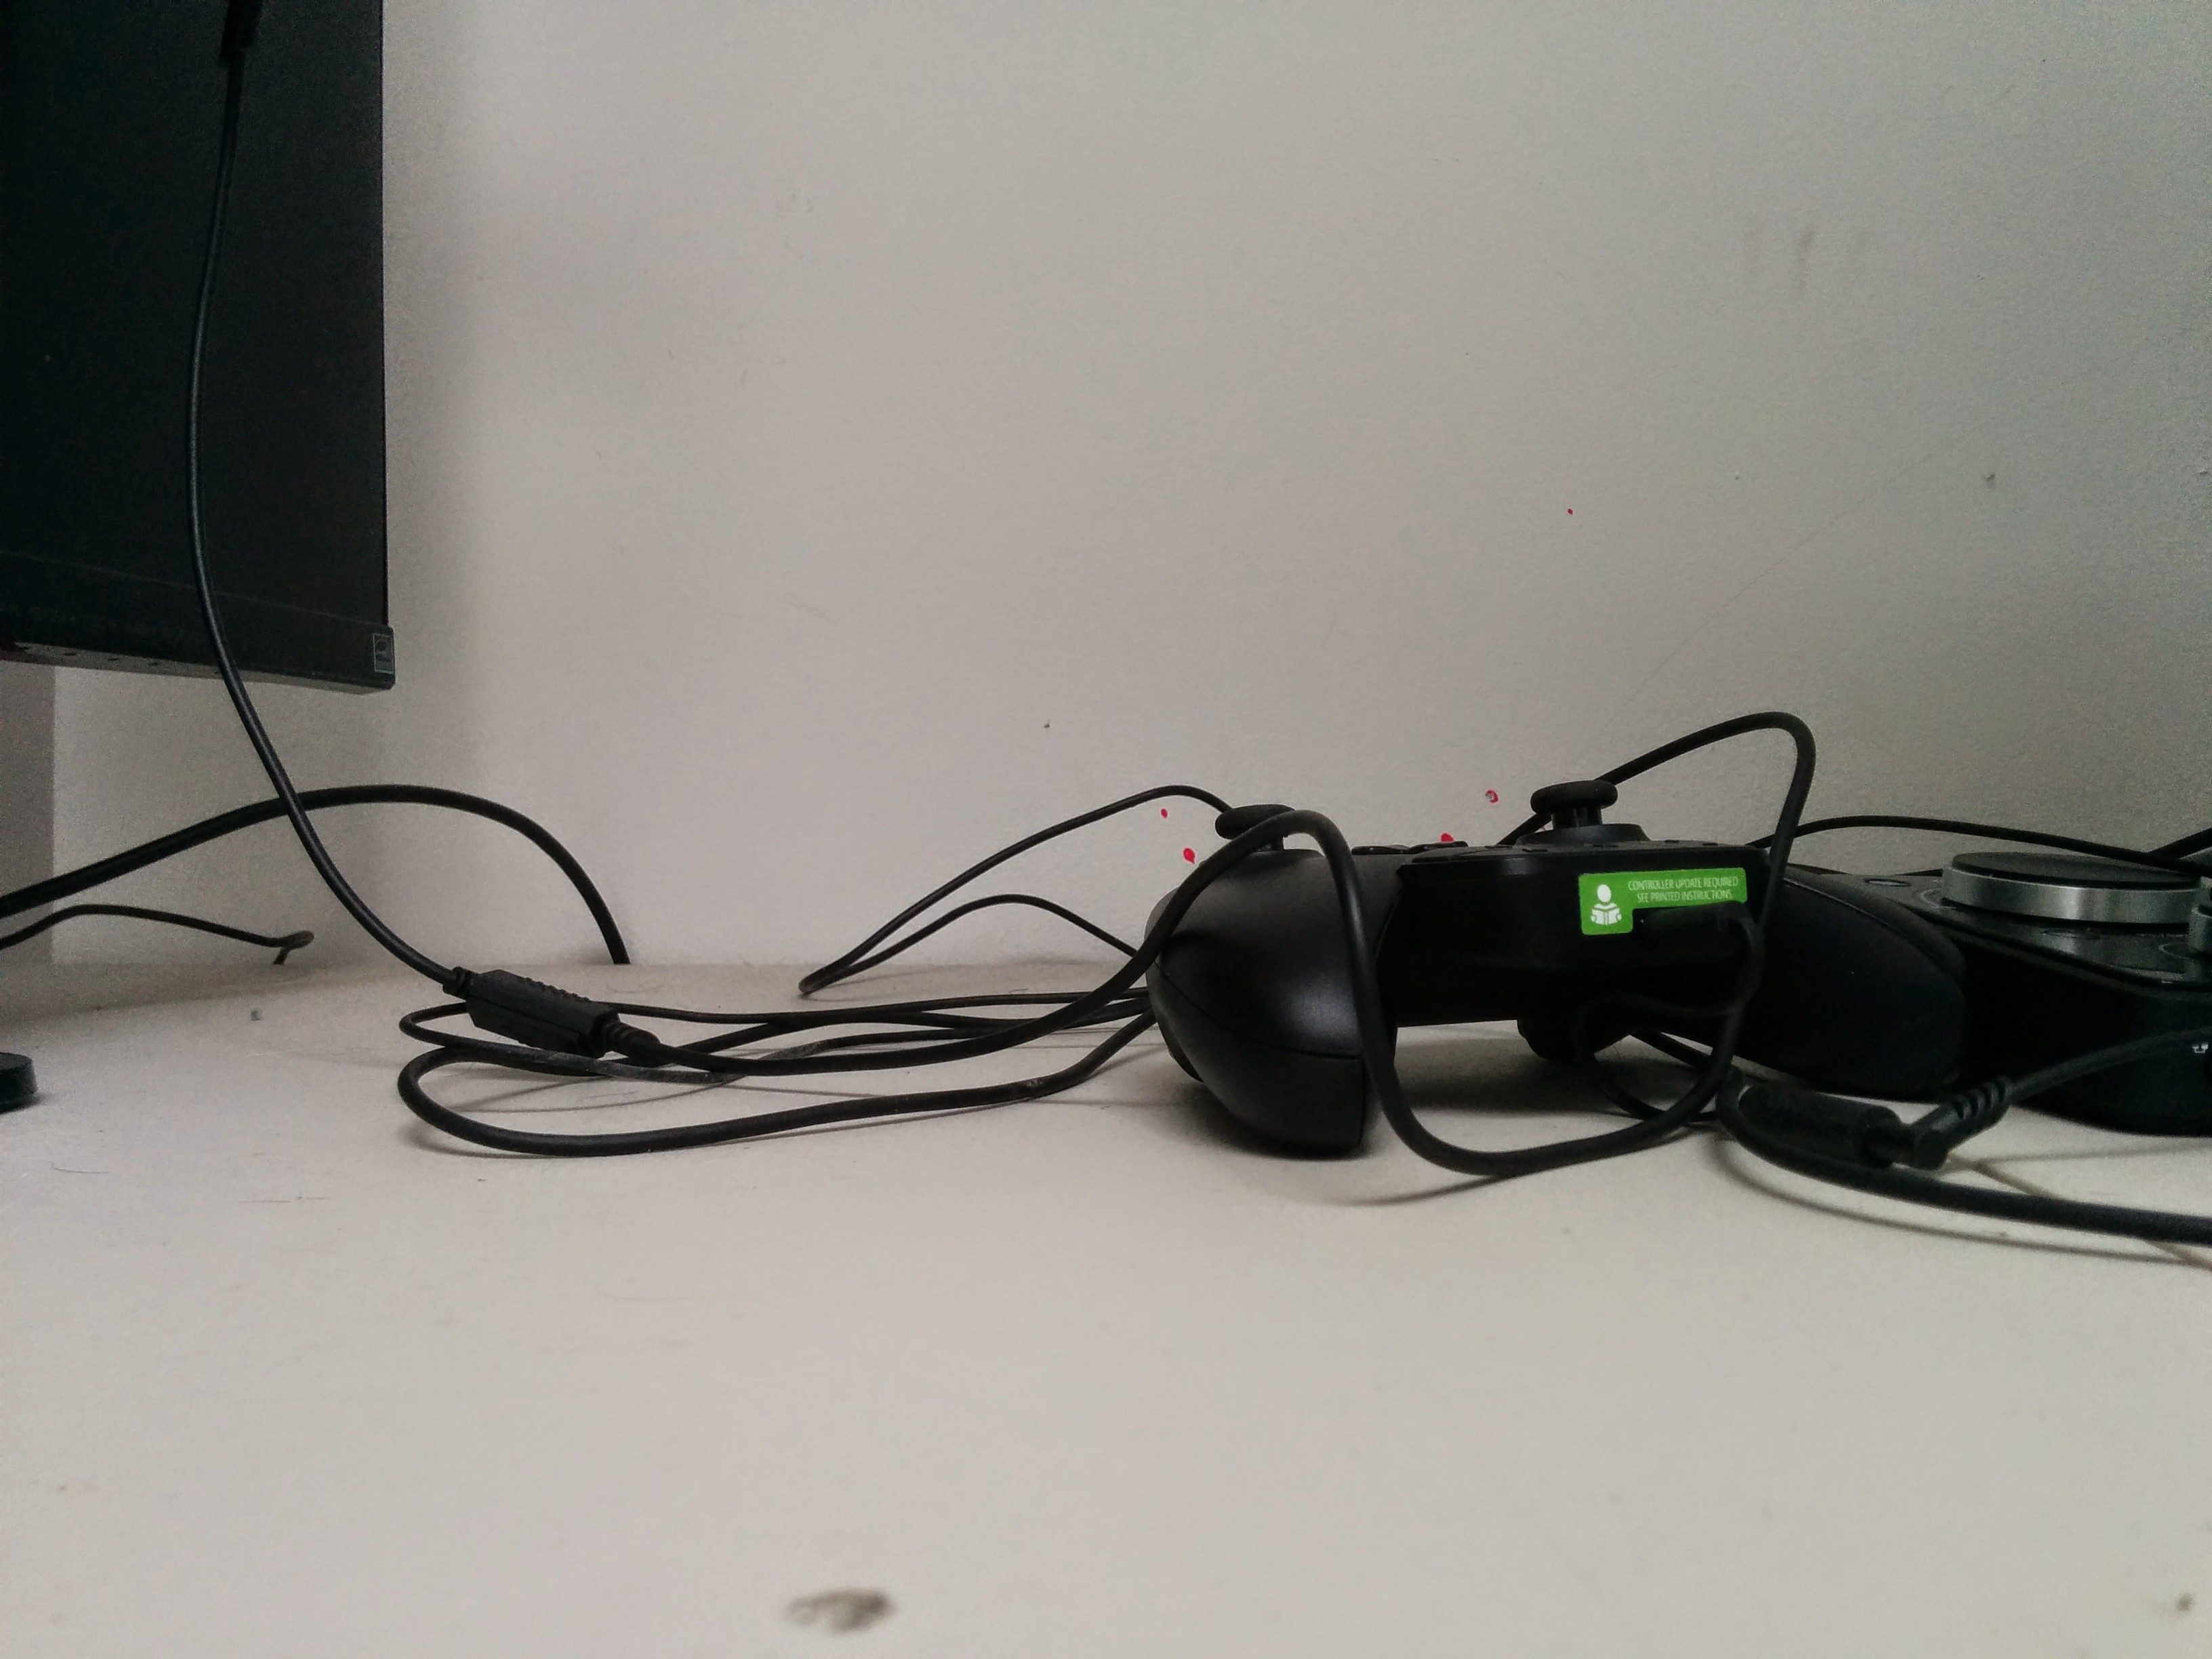
\includegraphics[width=\textwidth]{my-images/b2.jpg}
                \caption{Background 2}
                \label{fig:1b}
        \end{subfigure}
        \caption{Background input images}\label{fig:dataset}
\end{figure}

%c1 and c2
\begin{figure}[h!]
        \centering
        \begin{subfigure}[b]{0.49\textwidth}
                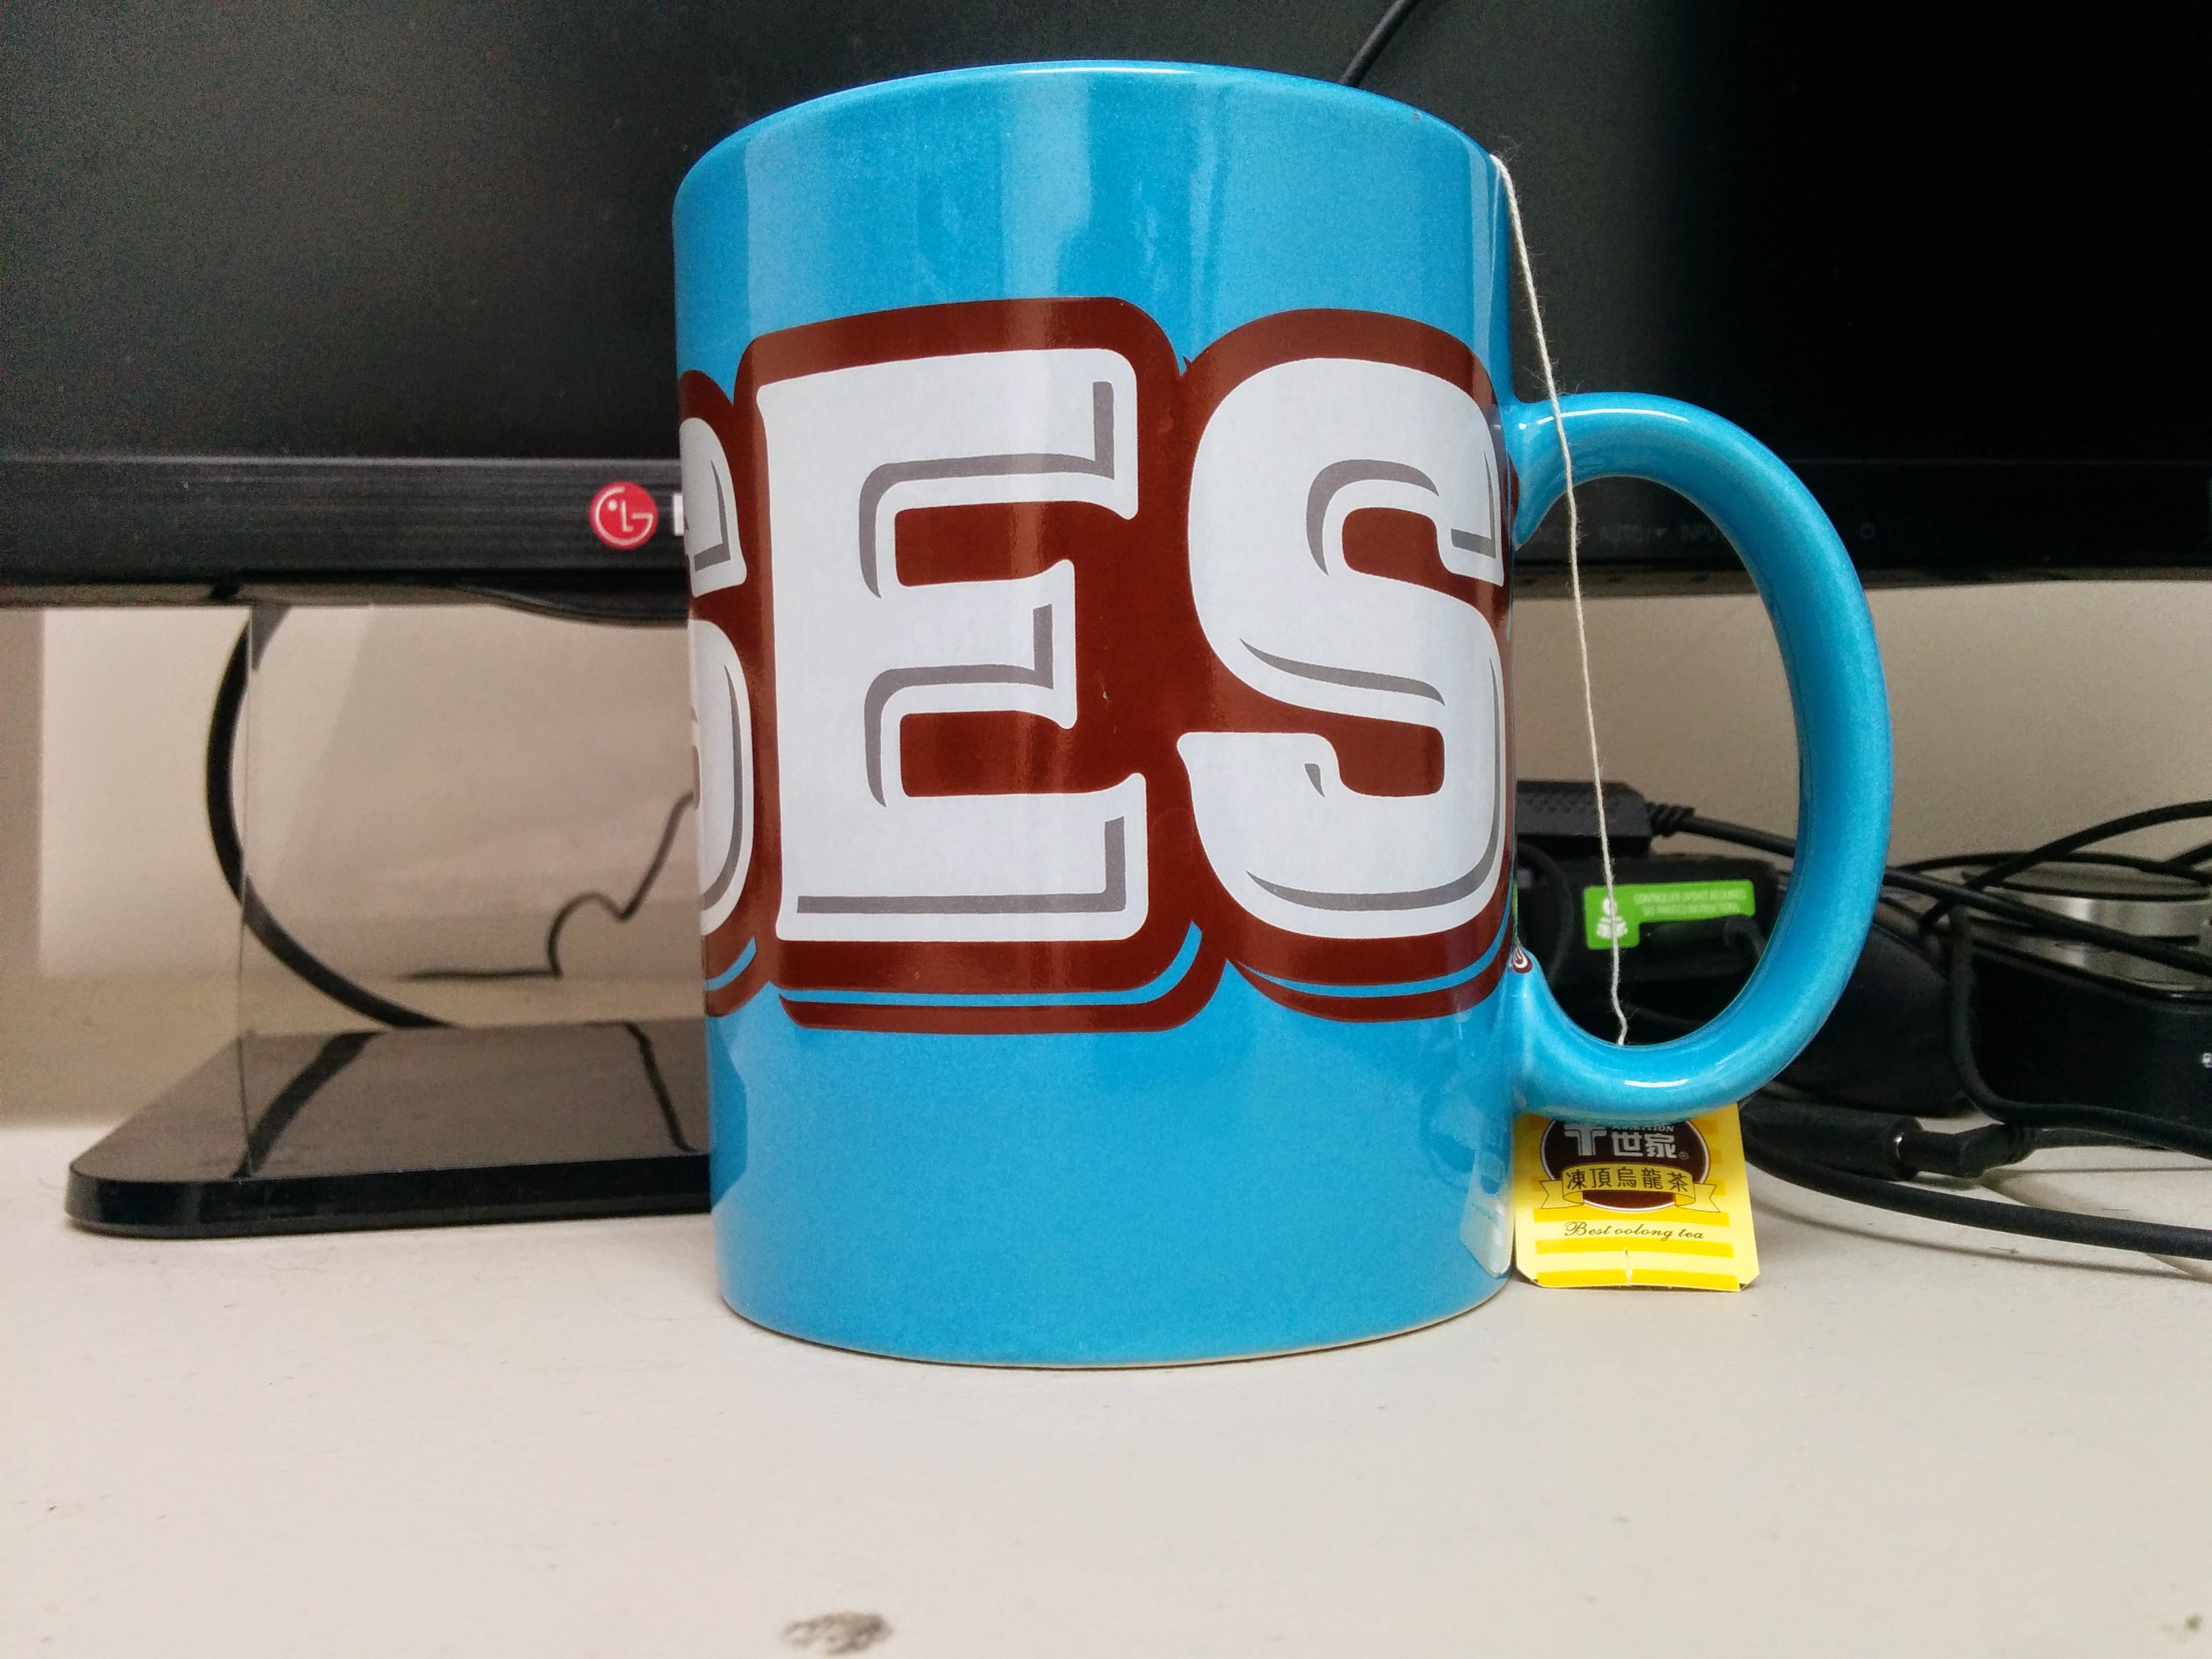
\includegraphics[width=\textwidth]{my-images/c1.jpg}
                \caption{Composite 1, (includes b1)}
                \label{fig:1a}
        \end{subfigure}%
        ~
        \begin{subfigure}[b]{0.49\textwidth}
                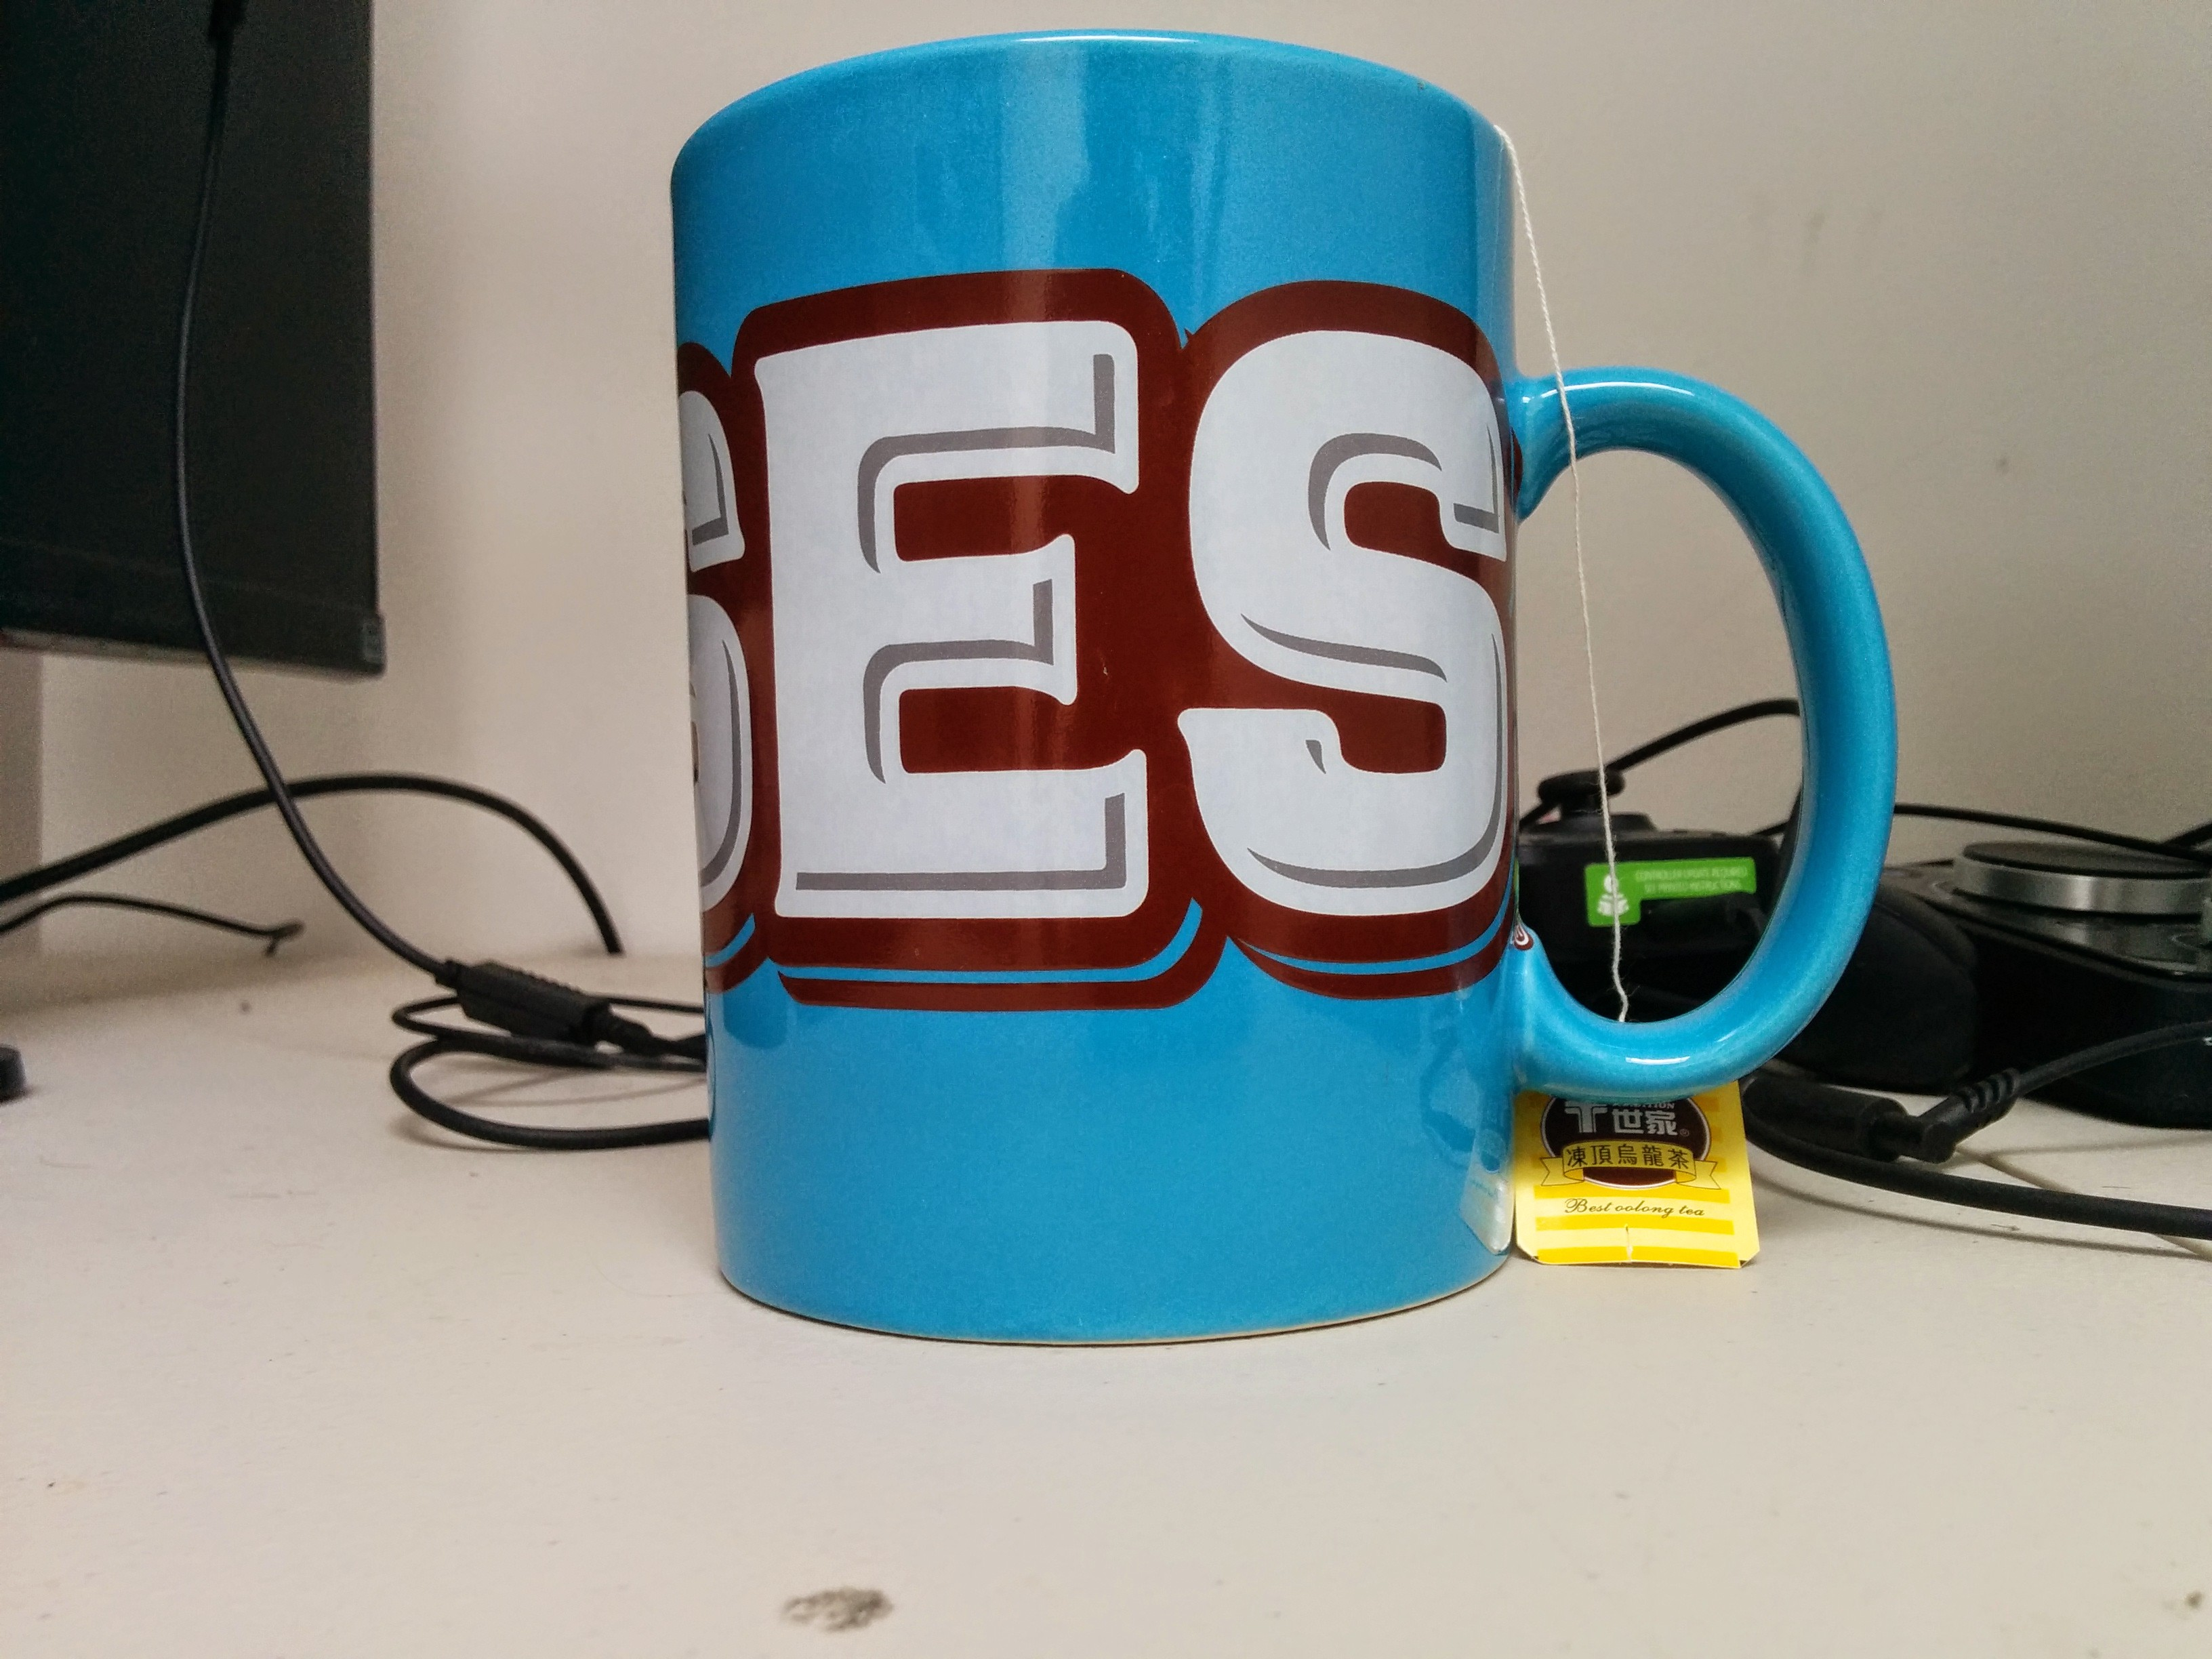
\includegraphics[width=\textwidth]{my-images/c2.jpg}
                \caption{Composite 2, (includes b2)}
                \label{fig:1b}
        \end{subfigure}
        \caption{Composite input images}\label{fig:dataset}
\end{figure}

\begin{figure}[h!]
        \centering
        \begin{subfigure}[b]{0.75\textwidth}
                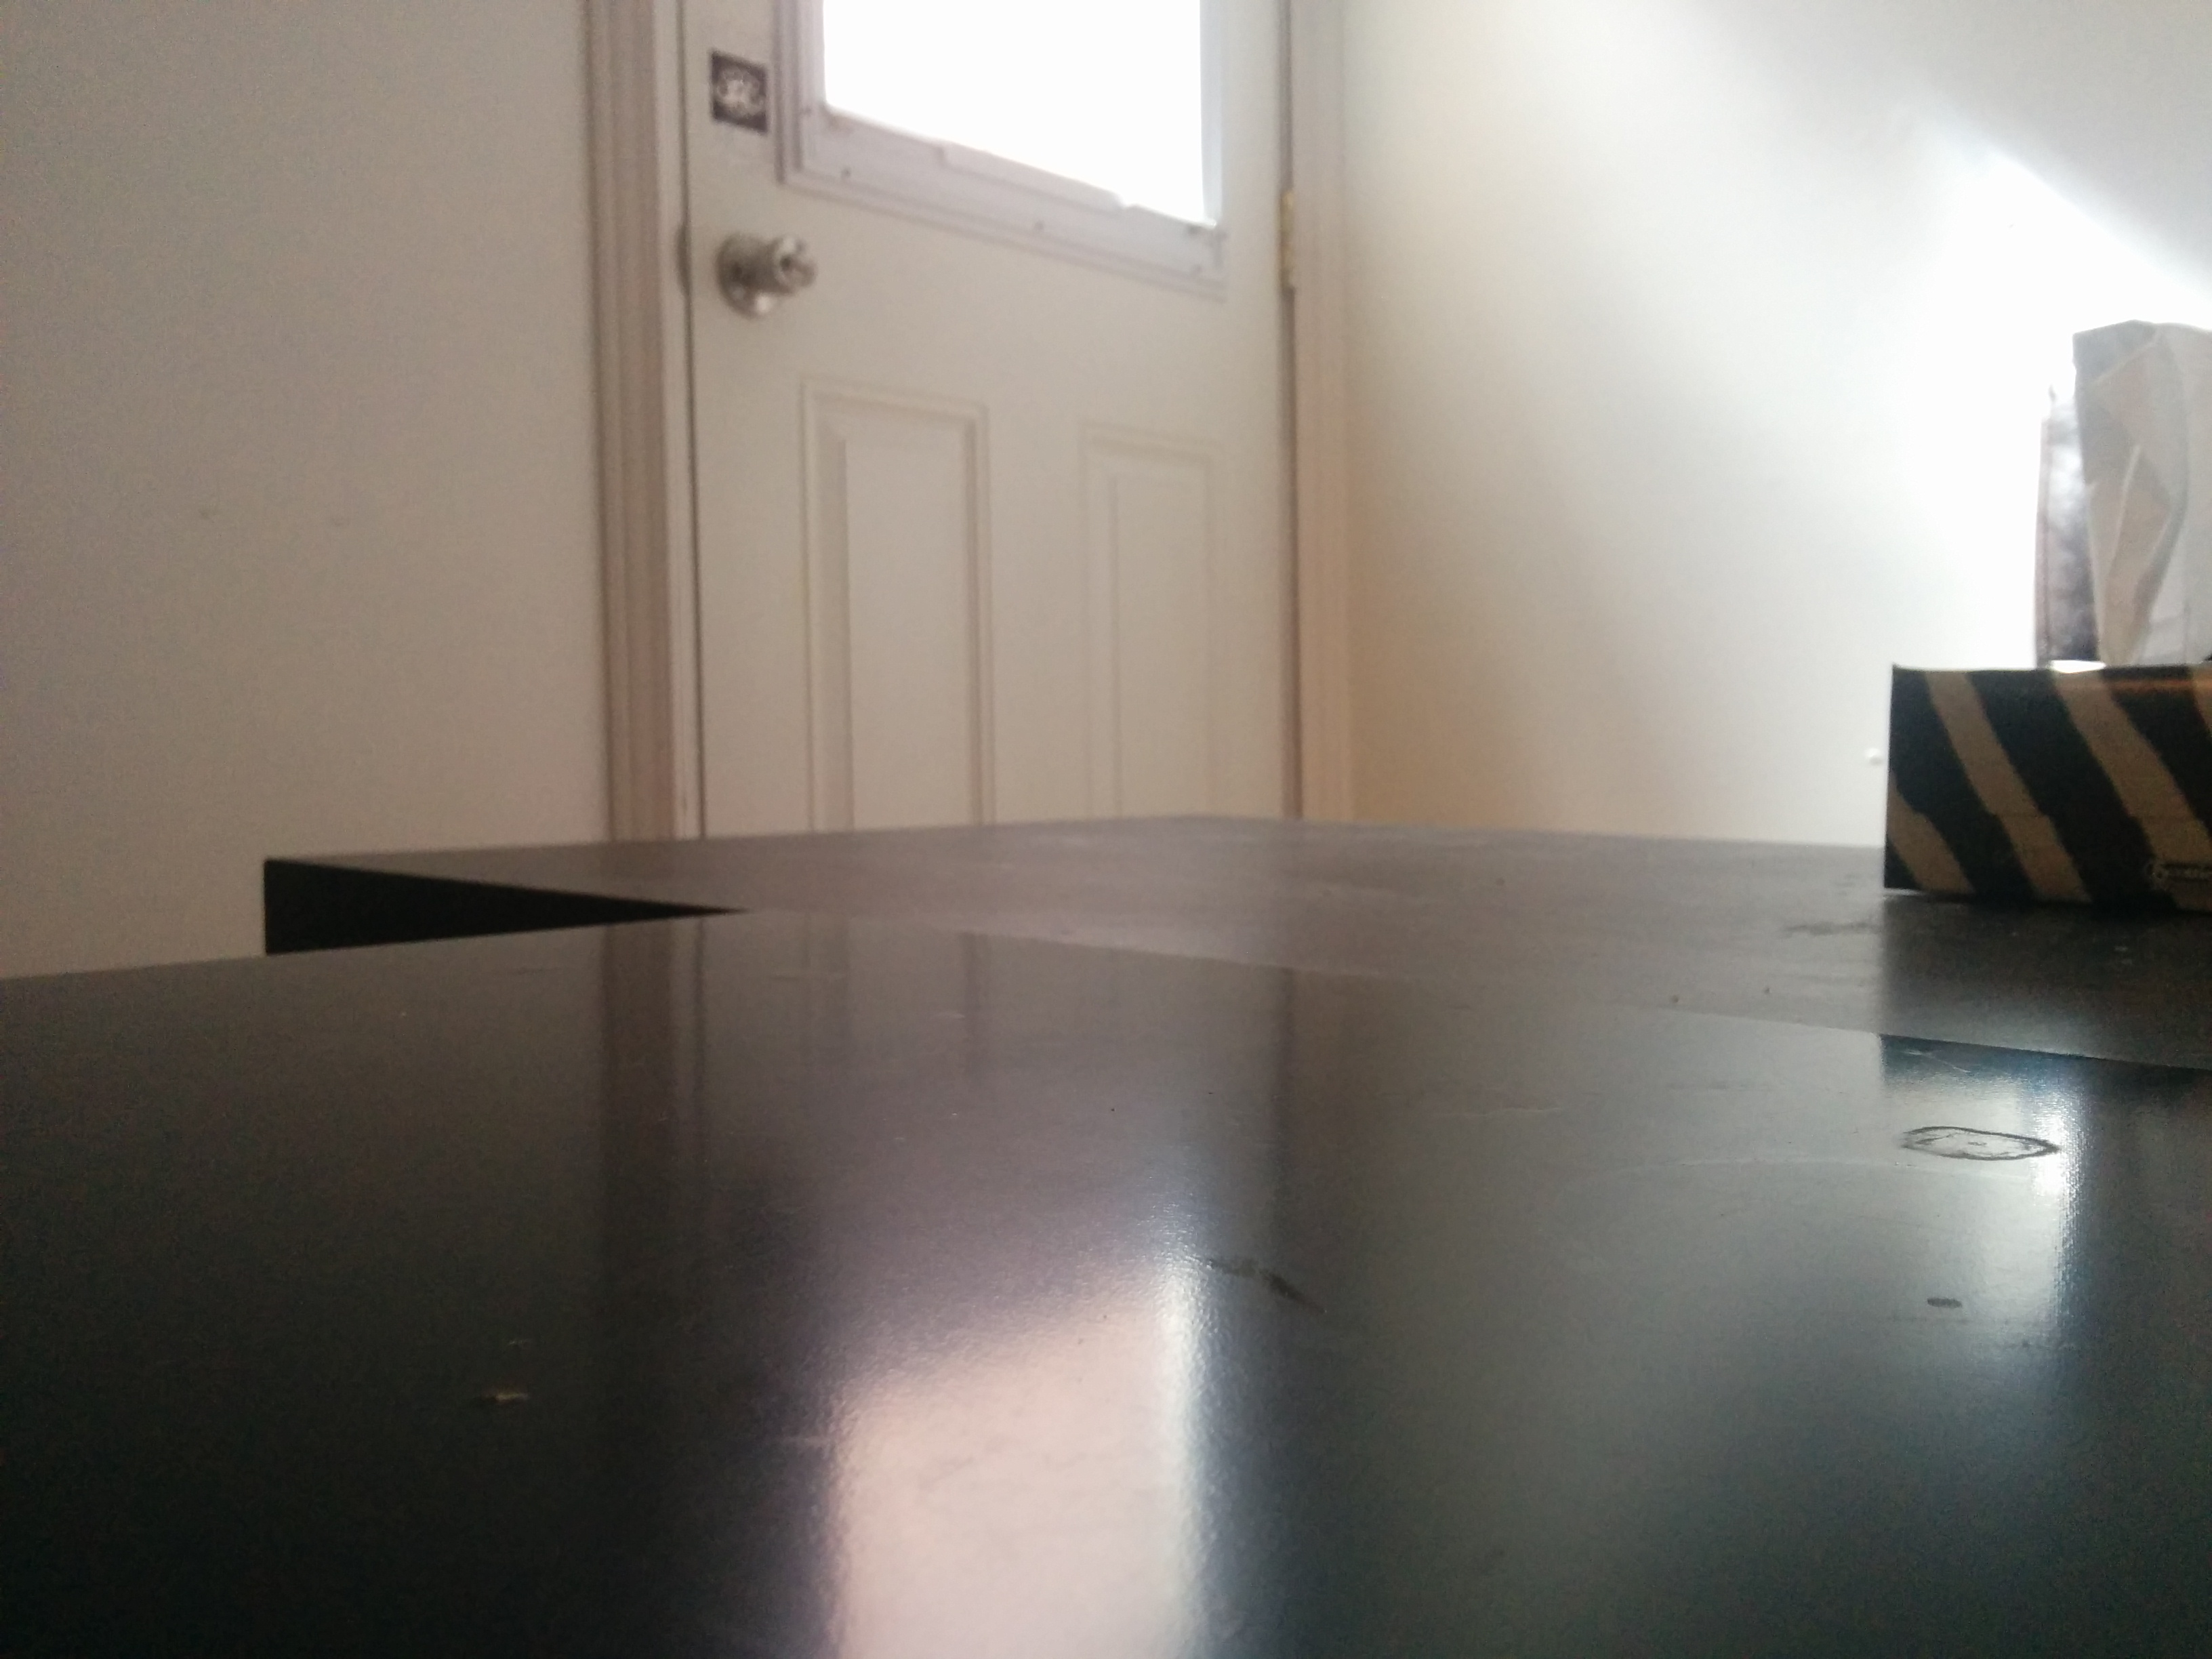
\includegraphics[width=\textwidth]{my-images/new-b.jpg}
                \caption{A background we want to combine with the mug (foreground object) in the two images directly above.}
                \label{fig:1a}
        \end{subfigure}%
        \caption{New background input image}\label{fig:dataset}
\end{figure}

Now for the results of the triangulation matting algorithm:

\begin{figure}[h!]
        \centering
        \begin{subfigure}[b]{0.49\textwidth}
                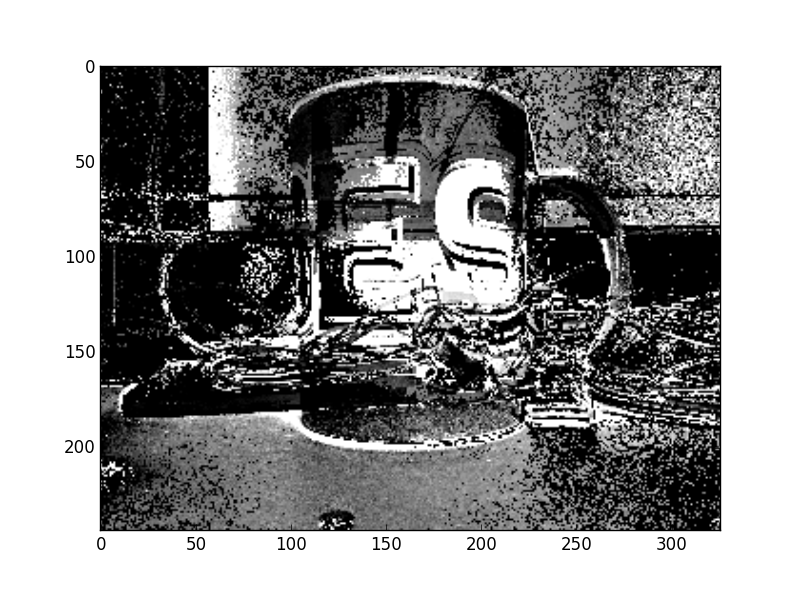
\includegraphics[width=\textwidth]{my-alpha.png}
                \caption{Alpha image computed with the images in Figure 2 and 3.}
                \label{fig:1a}
        \end{subfigure}%
        ~
        \begin{subfigure}[b]{0.49\textwidth}
                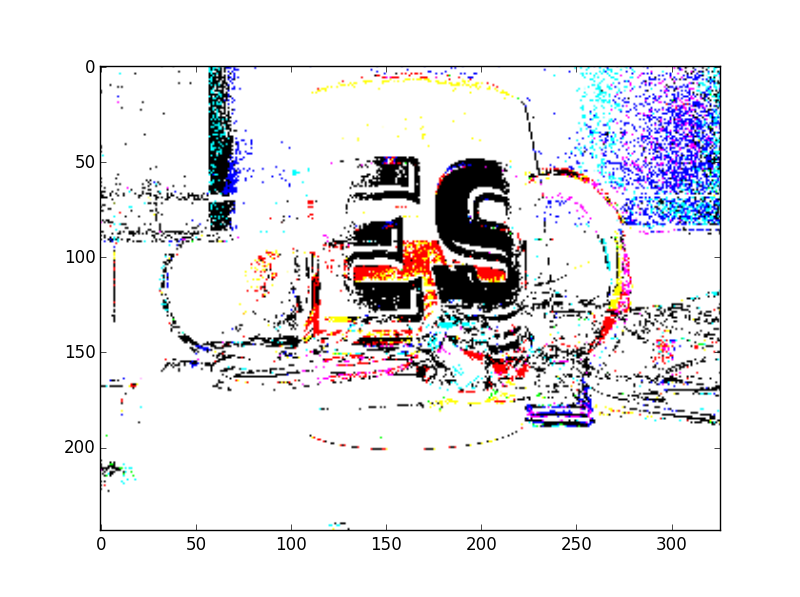
\includegraphics[width=\textwidth]{my-f.png}
                \caption{Foreground image computed with the images in Figure 2 and 3.}
                \label{fig:1b}
        \end{subfigure}
        \caption{Composite input images}\label{fig:dataset}
\end{figure}

\begin{figure}[h!]
        \centering
        \begin{subfigure}[b]{0.75\textwidth}
                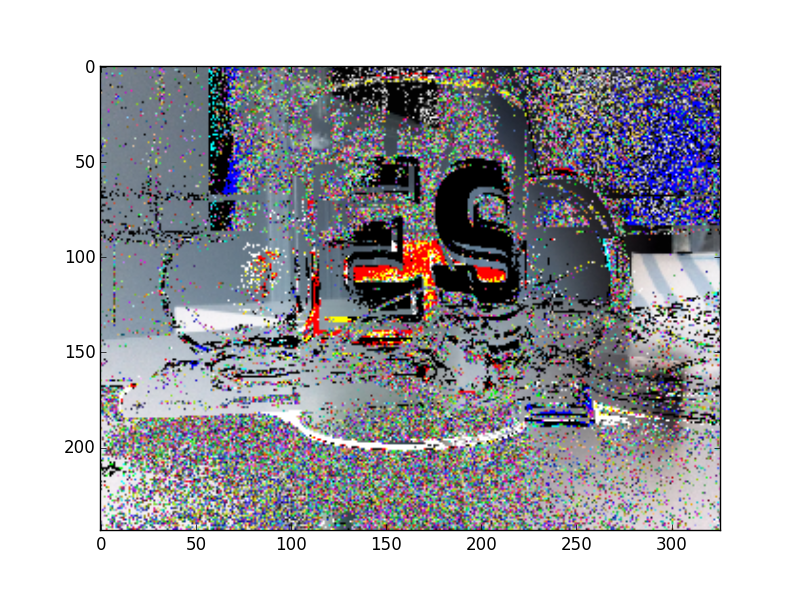
\includegraphics[width=\textwidth]{my-new-c.png}
                \caption{The new composite image produced by doing triangulation matting with figure 4 and 5. Pretty lousy results eh? Blame the output of these input images on my lack of skills as a photographer, not a computer scientist!
                }
                \label{fig:1a}
        \end{subfigure}%
        \caption{New background input image}\label{fig:dataset}
\end{figure}


\end{homeworkProblem}

\clearpage

\section{p4.py:}
\begin{lstlisting}
from pylab import *
import numpy as np
import random
import matplotlib.cbook as cbook
import random
import time
from scipy.misc import imread
from scipy.misc import imsave
from scipy.misc import imresize
import matplotlib.image as mpimg
import matplotlib.pyplot as plt
import os

matplotlib
gray()

os.chdir('C:/Users/Ramaneek/SkyDrive/Documents/Github/CSC320-Winter-2014/project 4/')

# c = f + (1-alpha)b

## MAIN
b1 = imread('images/flowers-backA.jpg')/255.0
c1 = imread('images/flowers-compA.jpg')/255.0
b2 = imread('images/flowers-backB.jpg')/255.0
c2 = imread('images/flowers-compB.jpg')/255.0
new_b = imread('images/window.jpg')/255.0

print "Read the input images"

new_c = np.zeros(new_b.shape)
alpha = np.zeros((b1.shape[0], b1.shape[1]))
f = np.zeros(b1.shape)

for i in range(b1.shape[0]):
    for j in range(b2.shape[1]):
        #set A
        A = np.matrix([ [1,0,0,-b1[i,j,0]], 
                        [0,1,0,-b1[i,j,1]], 
                        [0,0,1,-b1[i,j,2]], 
                        [1,0,0,-b2[i,j,0]], 
                        [0,1,0,-b2[i,j,1]], 
                        [0,0,1,-b2[i,j,2]] ])
                        
        #get the pseudo inverse of A
        A_pinv = linalg.pinv(A)
        
        #set b
        b = np.matrix([ [c1[i,j,0]-b1[i,j,0]], 
                        [c1[i,j,1]-b1[i,j,1]], 
                        [c1[i,j,2]-b1[i,j,2]],
                        [c2[i,j,0]-b2[i,j,0]], 
                        [c2[i,j,1]-b2[i,j,1]], 
                        [c2[i,j,2]-b2[i,j,2]] ])
                        
        #solve for x by A^-1*b
        x = np.clip(dot(A_pinv,b), 0, 1)
        
        #set foreground
        for k in range(3):
            f[i,j,k] = x[k]
        
        #set alpha channel
        alpha[i,j] = x[3]
        
        #set new composite image
        for k in range(3):
            new_c[i,j,k] = f[i,j,k] + np.dot((1-alpha[i,j]), new_b[i,j,k])

print "Computed alpha channel and isolated the foreground"
figure(1)
imshow(alpha)
figure(2)
imshow(f)
figure(3)
imshow(new_c)

show()

            
\end{lstlisting}
\end{document}